\documentclass[aspectratio=169,10pt]{beamer}
\usetheme{skd}

\title[Pertemuan 1 -- Pendahuluan]{Pendahuluan dan Tinjauan Kontrol Kontinu}
\subtitle{Introduction and Review of Continuous-Time Control}
\author{Ir. Estiyanti Ekawati, M.T., Ph.D. \quad\textbar\quad Faqihza Mukhlish, S.T., M.T., Ph.D.}
\institute{Program Studi Teknik Fisika, Fakultas Teknologi Industri, Institut Teknologi Bandung}
\date{Pertemuan 1 \textbar\ Semester I 2026/2027}

\begin{document}

% ===========================================================================
\begin{frame}[plain,noframenumbering]
	\titlepage
\end{frame}

\begin{frame}{Agenda hari ini}
	\framesubtitle{Today's agenda}
	\begin{columns}[T]
		\begin{column}{0.55\textwidth}
			\begin{enumerate}
				\item \textbf{Kontrak kuliah} \en{-- course contract}\\
				      {\small capaian, peta semester, praktikum, penilaian}
				\item \textbf{Mengapa kontrol digital?} \en{-- why digital control?}\\
				      {\small struktur sistem kontrol digital, jenis sinyal}
				\item \textbf{Tinjauan kontrol kontinu} \en{-- review}\\
				      {\small model, respons, kestabilan, PID, penalaan heuristik}
				\item \textbf{Menuju kontrol diskrit} \en{-- towards discrete control}\\
				      {\small apa yang berubah saat komputer masuk ke kalang}
			\end{enumerate}
		\end{column}
		\begin{column}{0.4\textwidth}
			\begin{block}{Sub-CPMK S1}
				\small Menjelaskan struktur sistem kontrol digital dan meninjau kembali pemodelan, spesifikasi kinerja, serta pengontrol PID kontinu.\\[3pt]
				\en{Explain the structure of a digital control system and review continuous-time modelling, performance specifications, and PID control.}
			\end{block}
		\end{column}
	\end{columns}
\end{frame}

% ===========================================================================
\section{Kontrak Kuliah\texorpdfstring{\\[4pt]{\Large\en{Course Contract}}}{ / Course Contract}}
% ===========================================================================

\begin{frame}{Tentang mata kuliah ini}
	\framesubtitle{About this course}
	\begin{columns}[T]
		\begin{column}{0.58\textwidth}
			Kuliah ini mempersiapkan Anda untuk \alert{merancang} sistem kontrol diskrit dengan metode \textbf{heuristik} maupun \textbf{analitik}, lalu \alert{menerapkannya} pada \textbf{mikroprosesor} agar memenuhi kriteria kestabilan dan kinerja.

			\vspace{0.3cm}
			\en{You will learn to design discrete-time controllers using heuristic and analytical methods and implement them on microprocessors to meet stability and performance criteria.}
		\end{column}
		\begin{column}{0.38\textwidth}
			\begin{block}{Identitas}
				\small
				\textbf{TF4015} \textbar\ 3 SKS\\
				Kuliah $3\times 50$ menit/minggu\\
				Praktikum terintegrasi (Modul 0--4)\\
				Tugas besar berkelompok
			\end{block}
		\end{column}
	\end{columns}
\end{frame}

\begin{frame}{Capaian pembelajaran mata kuliah (CPMK)}
	\framesubtitle{Course learning outcomes}
	\footnotesize
	\renewcommand{\arraystretch}{1.15}
	\begin{tabular}{@{}l >{\raggedright\arraybackslash}p{6.8cm} >{\raggedright\arraybackslash}p{6.4cm}@{}}
		\toprule
		 & \textbf{Indonesia} & \textbf{\en{English}} \\
		\midrule
		1 & Mengidentifikasi fenomena kontrol diskrit dan merumuskan modelnya & \en{Identify discrete control phenomena and formulate their models} \\
		2 & Menganalisis kestabilan dan kinerja sistem kontrol diskrit secara sistematik & \en{Systematically analyse stability and performance} \\
		3 & Menerapkan metode heuristik dan analitik untuk merancang sistem kontrol diskrit sesuai kriteria kinerja standar internasional & \en{Apply heuristic and analytical design methods meeting international performance criteria} \\
		4 & Menggunakan perangkat lunak simulasi untuk analisis dan perancangan & \en{Use simulation software for analysis and design} \\
		5 & Mengimplementasikan rancangan pada perangkat mikroprosesor & \en{Implement designs on microprocessor hardware} \\
		\bottomrule
	\end{tabular}
\end{frame}

\begin{frame}{Peta semester}
	\framesubtitle{Semester map}
	\centering
	\begin{tikzpicture}[
			wk/.style={draw=skdblue,thick,fill=white,rounded corners=2pt,minimum width=1.62cm,minimum height=1.25cm,align=center,font=\scriptsize,text width=1.5cm},
			ex/.style={wk,fill=skdorange!20,draw=skdorange},
			lab/.style={fill=skdgreen,text=white,font=\tiny\bfseries,rounded corners=1pt,inner sep=1.5pt},
		]
		\foreach \i/\t [count=\c from 0] in {
				1/Pendahuluan \& review,
				2/Pencacahan \& ADC/DAC,
				3/Persamaan beda \& transf.\ Z,
				4/Fungsi transfer pulsa,
				5/Emulasi \& PID diskrit,
				6/Respons di bidang $z$,
				7/Kestabilan,
				8/\textbf{UTS}} {
				\ifnum\i=8
					\node[ex] (w\i) at (\c*1.75,0) {\t};
				\else
					\node[wk] (w\i) at (\c*1.75,0) {\t};
				\fi
				\node[font=\tiny\bfseries,text=skdgray,anchor=south] at (w\i.north) {Mg \i};
			}
		\foreach \i/\t [count=\c from 0] in {
				9/\textit{Root locus} bidang $z$,
				10/Resp.\ frekuensi \& \textit{deadbeat},
				11/Ruang keadaan diskrit,
				12/Penempatan kutub,
				13/Pengamat keadaan,
				14/LQR \& filter Kalman,
				15/Implementasi \& presentasi,
				16/\textbf{UAS}} {
				\ifnum\i=16
					\node[ex] (w\i) at (\c*1.75,-2.0) {\t};
				\else
					\node[wk] (w\i) at (\c*1.75,-2.0) {\t};
				\fi
				\node[font=\tiny\bfseries,text=skdgray,anchor=south] at (w\i.north) {Mg \i};
			}
		\node[wk,fill=skdlight] at (w1) {Pendahuluan \& review};
		\foreach \w/\m in {3/0,5/1,7/2,10/3,13/4}
			\node[lab,anchor=north] at ([yshift=2pt]w\w.south) {Modul \m};
		\node[lab,fill=skdorange,anchor=north] at ([yshift=2pt]w15.south) {Tugas Besar};
		% Keterangan
		\node[anchor=north west,font=\scriptsize,align=left] at ([yshift=-0.5cm]w9.south west) {%
			\tikz\node[lab]{Modul};\ praktikum \en{lab}\qquad
			\tikz\node[lab,fill=skdorange]{Tugas Besar};\ presentasi \en{project}\\[2pt]
			Mg 1--7: \textbf{dasar \& metode heuristik} \en{(foundations \& heuristic design)}\\
			Mg 9--15: \textbf{metode analitik \& ruang keadaan} \en{(analytical \& state-space design)}};
	\end{tikzpicture}
\end{frame}

\begin{frame}{Praktikum: satu kit untuk seluruh semester}
	\framesubtitle{Laboratory: one kit for the whole semester}
	\begin{columns}[c]
		\begin{column}{0.5\textwidth}
			\centering
			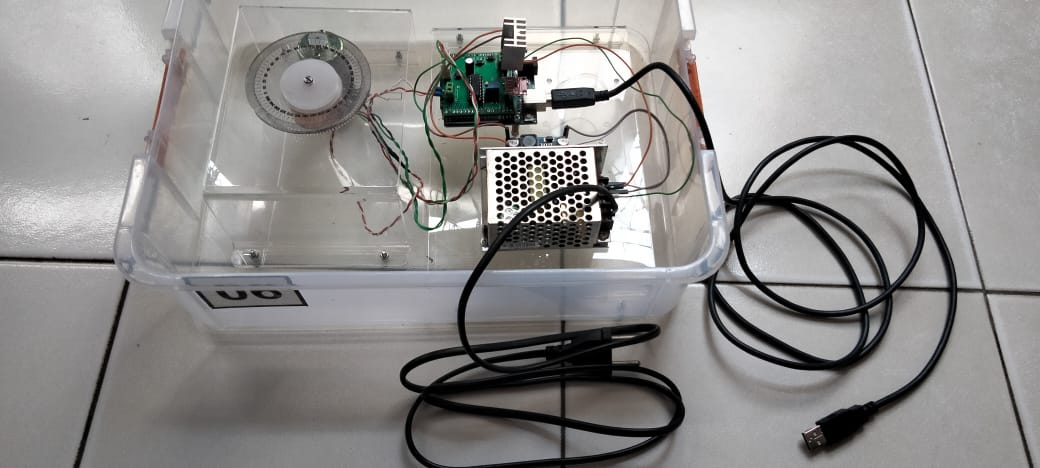
\includegraphics[width=\linewidth]{assets/kit_praktikum.jpg}\\[2pt]
			{\scriptsize\color{skdgray} Kit SKD: motor DC, tachometer, potensiometer, Arduino UNO + \textit{shield}, catu daya 24\,V}
		\end{column}
		\begin{column}{0.47\textwidth}
			\footnotesize
			\begin{tabular}{@{}c l c@{}}
				\toprule
				\textbf{Modul} & \textbf{Topik} & \textbf{Mg} \\
				\midrule
				0 & Pengenalan kit \en{(kit intro)} & 3 \\
				1 & Identifikasi sistem \en{(identification)} & 5 \\
				2 & Kontrol kecepatan \en{(speed)} & 7 \\
				3 & Kontrol posisi \en{(position)} & 10 \\
				4 & Penempatan kutub \en{(pole placement)} & 13 \\
				\bottomrule
			\end{tabular}

			\vspace{0.3cm}
			Setiap modul memakai hasil modul sebelumnya: \alert{model $\rightarrow$ pengontrol $\rightarrow$ uji}.
		\end{column}
	\end{columns}
\end{frame}

\begin{frame}{Tugas besar}
	\framesubtitle{Course project}
	\begin{columns}[T]
		\begin{column}{0.52\textwidth}
			Rancang, simulasikan, implementasikan, dan uji \textbf{satu metode kontrol diskrit selain PID konvensional} pada kit praktikum (kecepatan atau posisi):
			\begin{itemize}
				\item LQR \,/\, LQG
				\item \textit{Model Predictive Control} (MPC)
				\item \textit{Sliding Mode Control} (SMC)
				\item Penempatan kutub + pengamat + kriteria optimal
			\end{itemize}
			\vspace{0.1cm}
			{\small Diumumkan Mg 11, presentasi Mg 15 (10 menit + 5 menit tanya jawab).}
		\end{column}
		\begin{column}{0.44\textwidth}
			\footnotesize
			\begin{tabular}{@{}l r@{}}
				\toprule
				\textbf{Kriteria} & \textbf{Bobot} \\
				\midrule
				Kelengkapan dokumen & 30\% \\
				Pemahaman sistem \& metode & 30\% \\
				Hasil pengontrolan & 10\% \\
				Presentasi & 30\% \\
				Bonus (kreativitas, uji gangguan) & +15\% \\
				\bottomrule
			\end{tabular}
		\end{column}
	\end{columns}
\end{frame}

\begin{frame}{Penilaian dan ketentuan}
	\framesubtitle{Assessment and policies}
	% TODO: sesuaikan bobot dengan RPS final
	\begin{columns}[T]
		\begin{column}{0.4\textwidth}
			\begin{tikzpicture}
				\pgfmathsetmacro{\rr}{1.55}
				\def\slices{15/PR \& kuis/skdmid,20/Praktikum/skdgreen,15/Tugas besar/skdorange,25/UTS/skdblue,25/UAS/skdred}
				\def\start{90}
				\foreach \p/\n/\c in \slices {
						\pgfmathsetmacro{\e}{\start-\p*3.6}
						\fill[\c] (0,0) -- (\start:\rr) arc (\start:\e:\rr) -- cycle;
						\pgfmathsetmacro{\m}{(\start+\e)/2}
						\node[font=\scriptsize,text=white] at (\m:0.68*\rr) {\p\%};
						\node[font=\scriptsize,anchor={\m+180}] at (\m:\rr+0.08) {\n};
						\xdef\start{\e}
					}
				\fill[white] (0,0) circle (0.45);
			\end{tikzpicture}
		\end{column}
		\begin{column}{0.56\textwidth}
			\small
			\begin{itemize}
				\item Kehadiran kuliah $\geq 80\%$, praktikum 100\%.\\ \en{Attendance: lectures $\geq 80\%$, labs 100\%.}
				\item PR dikumpulkan via Edunex; terlambat dikenai pengurangan nilai.
				\item Diskusi dianjurkan, jawaban ditulis sendiri. Kode orang lain wajib diberi atribusi.
				\item Perangkat AI boleh untuk belajar dan pemrograman dengan menyebutkan penggunaannya; \alert{tidak boleh} saat kuis dan ujian.
				\item Kit dipakai sesuai SOP Modul 0.
			\end{itemize}
		\end{column}
	\end{columns}
\end{frame}

\begin{frame}{Buku teks dan perangkat lunak}
	\framesubtitle{Textbooks and software}
	\begin{columns}[T]
		\begin{column}{0.6\textwidth}
			\small
			\begin{description}
				\item[{[FR]}] Franklin, Powell, Emami-Naeini, \textit{Feedback Control of Dynamic Systems}, 8th ed., Pearson, 2018.
				\item[{[OG]}] Ogata, \textit{Discrete-Time Control Systems}, 2nd ed., Pearson India, 2015.
				\item[{[PH]}] Phillips, Nagle, Chakrabortty, \textit{Digital Control System Analysis \& Design}, 4th ed., Pearson, 2014.
			\end{description}
		\end{column}
		\begin{column}{0.36\textwidth}
			\begin{block}{Perangkat lunak}
				\small
				MATLAB/Simulink \textit{atau} Python (\texttt{numpy}, \texttt{scipy.signal}, \texttt{python-control})\\[3pt]
				Arduino IDE + \textit{library} Adafruit MCP4725
			\end{block}
			\vspace{0.15cm}
			{\small Bacaan pertemuan ini: [FR] Bab 1, 3, 4.3; [OG] 1.1--1.3}
		\end{column}
	\end{columns}
\end{frame}

% ===========================================================================
\section{Mengapa Kontrol Digital?\texorpdfstring{\\[4pt]{\Large\en{Why Digital Control?}}}{ / Why Digital Control?}}
% ===========================================================================

\begin{frame}{Kontrol digital ada di mana-mana}
	\framesubtitle{Digital control is everywhere}
	\begin{columns}[T]
		\begin{column}{0.48\textwidth}
			\begin{itemize}
				\item \textbf{Drone dan robot}: pengontrol penerbangan memperbarui aksi motor ratusan hingga ribuan kali per detik.
				\item \textbf{Penggerak motor dan servo}: robot industri, CNC, pencetak 3D.
				\item \textbf{Kontrol proses}: DCS dan PLC di kilang, pembangkit, dan pabrik; waktu cacah orde detik.
				\item \textbf{Otomotif}: ECU mesin, ABS, \textit{cruise control}.
			\end{itemize}
		\end{column}
		\begin{column}{0.48\textwidth}
			\begin{block}{Pola yang sama}
				\small
				Sensor dibaca \alert{pada saat tertentu}, komputer menghitung aksi kontrol, lalu aksi itu \alert{ditahan} hingga perhitungan berikutnya.\\[4pt]
				\en{Sensors are read at discrete instants, a computer computes the control action, and the action is held until the next update.}
			\end{block}
		\end{column}
	\end{columns}
\end{frame}

\begin{frame}{Struktur sistem kontrol digital}
	\framesubtitle{Structure of a digital control system}
	\centering
	\begin{tikzpicture}[node distance=0.55cm and 0.75cm]
		\node[sum] (s) {};
		\node[left=0.7cm of s] (r) {$r[k]$};
		\node[blkd,right=of s] (c) {Kontroler\\$D(z)$};
		\node[blk,right=1.1cm of c] (dac) {DAC\\+ ZOH};
		\node[blk,right=1.0cm of dac] (p) {Aktuator\\+ Plant $G(s)$};
		\node[right=1.1cm of p] (y) {$y(t)$};
		\node[blk,below=0.9cm of p] (sen) {Sensor};
		\node[blk] (adc) at (dac |- sen) {ADC};
		\draw[sig] (r) -- (s);
		\draw[sig] (s) -- node[above,lbl]{$e[k]$} (c);
		\draw[sig] (c) -- node[pos=0.68,above,lbl]{$u[k]$} (dac);
		\draw[sig] (dac) -- node[above,lbl]{$u(t)$} (p);
		\draw[sig] (p) -- coordinate[pos=0.5](yt) (y);
		\draw[sig] (yt) |- (sen);
		\draw[sig] (sen) -- node[above,lbl]{$y_m(t)$} (adc);
		\draw[sig] (adc) -| node[pos=0.25,above,lbl]{$y[k]$} node[pos=0.95,left,lbl]{$-$} (s);
		% komputer
		\node[draw=skdorange,dashed,thick,rounded corners,fit=(s)(c),inner sep=0.35cm,label={[font=\scriptsize\bfseries,text=skdorange]above:Komputer / mikrokontroler}] {};
		% jam
		\node[draw=skdgray,circle,inner sep=1pt,font=\scriptsize] (clk) at ($(dac)!0.5!(adc)$) {$T$};
		\draw[-{Stealth[length=1.6mm]},skdgray,dashed] (clk) -- (dac);
		\draw[-{Stealth[length=1.6mm]},skdgray,dashed] (clk) -- (adc);
		\node[lbl,right=0.05cm of clk] {jam cacah \en{(clock)}};
		% gangguan
		\node[above=0.5cm of p,lbl] (d) {gangguan $d(t)$};
		\draw[sig,skdgray] (d) -- (p);
	\end{tikzpicture}

	\vspace{0.25cm}
	{\small Dua dunia bertemu: sinyal \textbf{kontinu} $u(t), y(t)$ di plant dan sinyal \textbf{diskrit} $u[k], y[k]$ di komputer, dihubungkan oleh ADC dan DAC setiap \term{waktu cacah}{sampling period} $T$.}
\end{frame}

\begin{frame}{Pada kit praktikum}
	\framesubtitle{On the lab kit}
	\footnotesize
	\renewcommand{\arraystretch}{1.3}
	\begin{tabular}{@{}p{2.3cm} p{6.0cm} p{4.9cm}@{}}
		\toprule
		\textbf{Blok} & \textbf{Komponen pada kit SKD} & \textbf{Catatan} \\
		\midrule
		Kontroler $D(z)$ & Arduino UNO (ATmega328P, 16\,MHz) & program \texttt{loop()} dengan waktu cacah \texttt{millis()} \\
		DAC + ZOH & MCP4725 12-bit + OpAmp + TIP41C + L293D & nilai ditahan hingga cacah berikutnya \\
		Aktuator + plant & Motor DC COPAL 24\,V & \textit{deadzone} dan saturasi \\
		Sensor & Tachometer (kecepatan), potensiometer (posisi) & tachometer melalui filter RC \\
		ADC & ADC 10-bit Arduino, 0--5\,V & resolusi $\approx 4{,}9$\,mV \\
		\bottomrule
	\end{tabular}

	\vspace{0.4cm}
	\kunci{Setiap konsep di kuliah ini akan Anda temui kembali secara fisik di kit: pencacahan (Modul 0), model (Modul 1), PID diskrit (Modul 2--3), ruang keadaan (Modul 4).}
\end{frame}

\begin{frame}{Sinyal kontinu, diskrit, dan digital}
	\framesubtitle{Continuous, discrete-time, and digital signals}
	\begin{columns}[T]
		\begin{column}{0.32\textwidth}
			\centering
			\begin{tikzpicture}
				\begin{axis}[skd,width=5.2cm,height=3.6cm,xmin=0,xmax=6,ymin=-1.3,ymax=1.3,xlabel={$t$},ytick=\empty,xtick=\empty,title={\small Kontinu},title style={yshift=-4pt}]
					\addplot[skdblue,domain=0:6,samples=120] {sin(deg(1.2*x))+0.15*sin(deg(4*x))};
				\end{axis}
			\end{tikzpicture}\\
			{\scriptsize terdefinisi untuk setiap $t$\\\en{defined for all $t$}}
		\end{column}
		\begin{column}{0.32\textwidth}
			\centering
			\begin{tikzpicture}
				\begin{axis}[skd,width=5.2cm,height=3.6cm,xmin=0,xmax=6,ymin=-1.3,ymax=1.3,xlabel={$k$},ytick=\empty,xtick=\empty,title={\small Diskrit (tercacah)},title style={yshift=-4pt}]
					\addplot[skdblue!35,domain=0:6,samples=120,thin] {sin(deg(1.2*x))+0.15*sin(deg(4*x))};
					\addplot[skdorange,ycomb,mark=*,mark size=1.2pt,samples at={0,0.4,...,6}] {sin(deg(1.2*x))+0.15*sin(deg(4*x))};
				\end{axis}
			\end{tikzpicture}\\
			{\scriptsize hanya pada $t = kT$, amplitudo kontinu\\\en{only at $t=kT$, continuous amplitude}}
		\end{column}
		\begin{column}{0.32\textwidth}
			\centering
			\begin{tikzpicture}
				\begin{axis}[skd,width=5.2cm,height=3.6cm,xmin=0,xmax=6,ymin=-1.3,ymax=1.3,xlabel={$t$},ytick={-1,-0.5,...,1},yticklabels={},xtick=\empty,title={\small Digital + ZOH},title style={yshift=-4pt}]
					\addplot[skdblue!35,domain=0:6,samples=120,thin] {sin(deg(1.2*x))+0.15*sin(deg(4*x))};
					\addplot[skdgreen,const plot,samples at={0,0.4,...,6.4}] {round(2*(sin(deg(1.2*x))+0.15*sin(deg(4*x))))/2};
				\end{axis}
			\end{tikzpicture}\\
			{\scriptsize waktu \emph{dan} amplitudo terkuantisasi\\\en{quantised in time and amplitude}}
		\end{column}
	\end{columns}
	\vspace{0.35cm}
	\kunci{Pencacahan \en{(sampling)} dan kuantisasi \en{(quantisation)} dibahas rinci pada Pertemuan 2.}
\end{frame}

\begin{frame}{Analog atau digital?}
	\framesubtitle{Analog or digital?}
	\begin{columns}[T]
		\begin{column}{0.48\textwidth}
			\begin{exampleblock}{Keunggulan kontrol digital}
				\small
				\begin{itemize}
					\item Algoritma diubah lewat perangkat lunak, bukan rangkaian
					\item Algoritma kompleks: logika, estimasi, optimasi, adaptif
					\item Tidak ada \textit{drift} komponen; mudah direplikasi
					\item Pencatatan data, komunikasi, dan diagnosis
				\end{itemize}
			\end{exampleblock}
		\end{column}
		\begin{column}{0.48\textwidth}
			\begin{alertblock}{Konsekuensi yang harus dikelola}
				\small
				\begin{itemize}
					\item Informasi hilang di antara cacah; risiko \textit{aliasing}
					\item ZOH dan waktu komputasi menambah \alert{tunda}
					\item Kuantisasi ADC/DAC dan presisi aritmetika
					\item Perlu alat analisis baru: \textbf{transformasi Z}, bidang $z$
				\end{itemize}
			\end{alertblock}
		\end{column}
	\end{columns}
\end{frame}

% ===========================================================================
\section{Tinjauan Kontrol Kontinu\texorpdfstring{\\[4pt]{\Large\en{Review of Continuous Control}}}{ / Review of Continuous Control}}
% ===========================================================================

\begin{frame}{Apa tujuan sistem kontrol?}
	\framesubtitle{What is a control system for?}
	\begin{columns}[T]
		\begin{column}{0.5\textwidth}
			\term{Kontrol}{control}: upaya memastikan suatu sistem berperilaku sesuai kriteria perancangannya.

			\vspace{0.3cm}
			\centering
			\begin{tikzpicture}[node distance=0.45cm and 0.5cm]
				\node[sum] (s) {};
				\node[left=0.45cm of s,font=\small] (r) {$r$};
				\node[blkd,right=of s,minimum width=1.1cm] (c) {$C(s)$};
				\node[blk,right=of c,minimum width=1.1cm] (g) {$G(s)$};
				\node[right=0.5cm of g,font=\small] (y) {$y$};
				\draw[sig] (r) -- (s);
				\draw[sig] (s) -- node[above,lbl]{$e$} (c);
				\draw[sig] (c) -- node[above,lbl]{$u$} (g);
				\draw[sig] (g) -- coordinate[pos=0.4](m) (y);
				\draw[sig] (m) -- ++(0,-0.85) -| node[pos=0.9,left,lbl]{$-$} (s);
			\end{tikzpicture}
		\end{column}
		\begin{column}{0.46\textwidth}
			\textbf{Kriteria perancangan} \en{(design criteria)}
			\begin{enumerate}
				\item \term{Kestabilan}{stability}
				\item \term{Kecepatan respons}{speed}: $t_r$, $t_s$
				\item \term{Akurasi}{accuracy}: $M_p$, galat tunak
				\item \term{Ketegaran}{robustness}: terhadap galat model, gangguan, derau
			\end{enumerate}
			\vspace{0.1cm}
			{\small dengan batasan usaha kontrol $u$ (saturasi aktuator).}
		\end{column}
	\end{columns}
\end{frame}

\begin{frame}{Pemodelan: contoh motor DC}
	\framesubtitle{Modelling example: DC motor}
	\begin{columns}[T]
		\begin{column}{0.5\textwidth}
			\small
			Hukum Kirchhoff (listrik) dan Newton (mekanik):
			\begin{align*}
				L\frac{di}{dt} + R\,i &= v - K\,\omega \\
				J\frac{d\omega}{dt} + b\,\omega &= K\,i
			\end{align*}
			Transformasi Laplace (kondisi awal nol):
			\[
				\frac{\Omega(s)}{V(s)} = \frac{K}{(Js+b)(Ls+R)+K^2}
			\]
		\end{column}
		\begin{column}{0.46\textwidth}
			\small
			Karena $L$ kecil, kutub listrik jauh lebih cepat sehingga
			\[
				\frac{\Omega(s)}{V(s)} \approx \frac{K_m}{\tau_m s + 1},\quad
				K_m = \frac{K}{bR+K^2},\ \ \tau_m = \frac{JR}{bR+K^2}
			\]
			\begin{block}{Langkah pemodelan}
				\scriptsize
				1) pahami sistem fisik,\ 2) tetapkan asumsi,\ 3) terapkan hukum dasar,\ 4) tulis persamaan diferensial,\ 5) linierisasi bila perlu.
			\end{block}
			{\scriptsize Pada Modul 1, $K_m$ dan $\tau_m$ diperoleh dari \textbf{data}, bukan dari parameter fisik.}
		\end{column}
	\end{columns}
\end{frame}

\begin{frame}{Fungsi transfer dan model generik}
	\framesubtitle{Transfer functions and generic process models}
	\small
	\term{Fungsi transfer}{transfer function}: $G(s) = Y(s)/U(s)$ dengan kondisi awal nol. Akar penyebut adalah \term{kutub}{poles}, akar pembilang adalah \term{zero}{zeros}.

	\vspace{0.25cm}
	\renewcommand{\arraystretch}{2.0}
	\begin{tabular}{@{}l l l l@{}}
		\toprule
		\textbf{Model} & \textbf{Persamaan diferensial} & \textbf{$G(s)$} & \textbf{Contoh} \\
		\midrule
		Orde 1 & $\tau\dot y + y = K u$ & $\dfrac{K}{\tau s+1}$ & kecepatan motor, suhu \\
		Integrator & $\dot y = K u$ & $\dfrac{K}{s}$ & posisi motor, level tangki \\
		Orde 2 & $\ddot y + 2\zeta\omega_n\dot y + \omega_n^2 y = K\omega_n^2 u$ & $\dfrac{K\omega_n^2}{s^2+2\zeta\omega_n s+\omega_n^2}$ & pegas--massa, servo \\
		FOPDT & $\tau\dot y(t) + y(t) = K u(t-\theta)$ & $\dfrac{K e^{-\theta s}}{\tau s+1}$ & proses industri \\
		\bottomrule
	\end{tabular}

	\vspace{0.25cm}
	{\footnotesize FOPDT = \en{first-order plus dead time}, model orde 1 dengan waktu tunda; dasar penalaan heuristik.}
\end{frame}

\begin{frame}{Respons tangga sistem orde 1}
	\framesubtitle{Step response of a first-order system}
	\begin{columns}[c]
		\begin{column}{0.55\textwidth}
			\centering
			\begin{tikzpicture}
				\begin{axis}[skd,width=8cm,height=5.2cm,xmin=0,xmax=5,ymin=0,ymax=1.1,xlabel={$t/\tau$},ylabel={$y/K$},xtick={0,1,2,3,4,5},ytick={0,0.632,1},yticklabels={0,$0{,}632$,$1$}]
					\addplot[skdblue,domain=0:5,samples=100] {1-exp(-x)};
					\addplot[skdorange,dashed,domain=0:1] {x};
					\draw[skdgray,dashed] (axis cs:1,0) -- (axis cs:1,0.632) -- (axis cs:0,0.632);
					\draw[skdgray,dashed] (axis cs:4,0) -- (axis cs:4,0.98);
					\node[font=\scriptsize,anchor=west] at (axis cs:1.05,0.55) {$63{,}2\%$ pada $t=\tau$};
					\node[font=\scriptsize,anchor=west] at (axis cs:4.05,0.45) {$98\%$};
					\node[font=\scriptsize,anchor=north] at (axis cs:4,0.38) {$t=4\tau$};
				\end{axis}
			\end{tikzpicture}
		\end{column}
		\begin{column}{0.42\textwidth}
			\[
				y(t) = K\left(1 - e^{-t/\tau}\right)\,u_0
			\]
			\begin{itemize}
				\item \term{Penguatan}{gain} $K$: nilai tunak per satuan masukan
				\item \term{Konstanta waktu}{time constant} $\tau$: waktu mencapai 63,2\%
				\item Waktu turun 2\%: $t_s \approx 4\tau$
				\item Garis singgung awal memotong nilai akhir di $t=\tau$
			\end{itemize}
		\end{column}
	\end{columns}
\end{frame}

\begin{frame}{Respons tangga orde 2 dan spesifikasi kinerja}
	\framesubtitle{Second-order step response and performance specifications}
	\begin{columns}[c]
		\begin{column}{0.55\textwidth}
			\centering
			% zeta = 0.4, wn = 2 rad/s
			\begin{tikzpicture}
				\pgfmathsetmacro{\z}{0.4}\pgfmathsetmacro{\wn}{2}
				\pgfmathsetmacro{\wdmp}{\wn*sqrt(1-\z^2)}\pgfmathsetmacro{\ph}{acos(\z)}
				\begin{axis}[skd,width=8cm,height=5.2cm,xmin=0,xmax=7,ymin=0,ymax=1.4,xlabel={$t$ (s)},ylabel={$y$},ytick={0,0.5,1,1.254},yticklabels={0,0.5,1,$1+M_p$}]
					\addplot[skdblue,domain=0:7,samples=200] {1-exp(-\z*\wn*x)/sqrt(1-\z^2)*sin(deg(\wdmp*x)+\ph)};
					\addplot[skdgray,dashed,thin,domain=0:7] {1.02};
					\addplot[skdgray,dashed,thin,domain=0:7] {0.98};
					\draw[skdorange,thick,<->] (axis cs:1.714,1) -- (axis cs:1.714,1.254) node[midway,right,font=\scriptsize]{$M_p$};
					\draw[skdgray,dashed] (axis cs:1.714,0) -- (axis cs:1.714,1);
					\node[font=\scriptsize,anchor=north] at (axis cs:1.714,0.25) {$t_p$};
					\draw[skdgray,dashed] (axis cs:4.9,0) -- (axis cs:4.9,0.98);
					\node[font=\scriptsize,anchor=north] at (axis cs:4.9,0.25) {$t_s$};
					\node[font=\scriptsize,anchor=west] at (axis cs:5.3,1.12) {pita $\pm 2\%$};
				\end{axis}
			\end{tikzpicture}\\
			{\scriptsize $\zeta=0{,}4$, $\omega_n=2$ rad/s}
		\end{column}
		\begin{column}{0.42\textwidth}
			\small
			Untuk $0<\zeta<1$, $\omega_d = \omega_n\sqrt{1-\zeta^2}$:
			\begin{align*}
				M_p &= e^{-\pi\zeta/\sqrt{1-\zeta^2}} \\
				t_p &= \pi/\omega_d \\
				t_r &\approx 1{,}8/\omega_n \quad (10\text{--}90\%) \\
				t_s &\approx 4/(\zeta\omega_n) \quad (2\%)
			\end{align*}
			\kunci{Spesifikasi $\rightarrow$ batas $\zeta$ dan $\zeta\omega_n$ $\rightarrow$ daerah kutub yang diinginkan.}
		\end{column}
	\end{columns}
\end{frame}

\begin{frame}{Lokasi kutub menentukan respons}
	\framesubtitle{Pole location determines the response}
	\begin{columns}[c]
		\begin{column}{0.5\textwidth}
			\centering
			\begin{tikzpicture}[scale=0.95]
				% daerah yang diinginkan: zeta >= 0.5 (sudut 60 derajat), sigma <= -1
				\fill[skdgreen!15] (-1,0) -- (-1,1.732) -- (-1.8,3.118) -- (-3.6,3.118) -- (-3.6,-3.118) -- (-1.8,-3.118) -- (-1,-1.732) -- cycle;
				\fill[skdred!8] (0,-3.1) rectangle (2.2,3.1);
				\draw[-{Stealth},thick] (-3.8,0) -- (2.4,0) node[right]{$\sigma$};
				\draw[-{Stealth},thick] (0,-3.2) -- (0,3.3) node[above]{$j\omega$};
				\draw[skdgreen!60!black,dashed] (0,0) -- (-1.8,3.118);
				\draw[skdgreen!60!black,dashed] (0,0) -- (-1.8,-3.118);
				\draw[skdgreen!60!black,dashed] (-1,-3.1) -- (-1,3.1);
				\draw[skdgray] (-0.6,0) arc (180:120:0.6);
				\node[font=\scriptsize,skdgray,anchor=south east] at (-0.55,0.45) {$\cos^{-1}\zeta$};
				\node[font=\scriptsize,text=skdgreen!50!black,align=center] at (-2.6,1.2) {daerah\\diinginkan};
				\node[font=\scriptsize,text=skdred,align=center] at (1.2,2.2) {tidak\\stabil};
				\node[font=\scriptsize,anchor=north] at (-1,-0.05) {$-\zeta\omega_n$};
				\foreach \x/\y in {-2/1.6,-2/-1.6} \node[skdblue,font=\large] at (\x,\y) {$\times$};
				\foreach \x/\y in {1/1.2,1/-1.2} \node[skdred,font=\large] at (\x,\y) {$\times$};
			\end{tikzpicture}
		\end{column}
		\begin{column}{0.46\textwidth}
			\small
			Kutub $s = -\zeta\omega_n \pm j\omega_d$:
			\begin{itemize}
				\item bagian riil $-\zeta\omega_n$ $\rightarrow$ laju peluruhan, $t_s$
				\item bagian imajiner $\omega_d$ $\rightarrow$ frekuensi osilasi
				\item sudut terhadap sumbu riil negatif $\rightarrow$ $\zeta$, $M_p$
				\item bagian riil positif $\rightarrow$ \alert{tidak stabil}
			\end{itemize}
			\vspace{0.15cm}
			\begin{block}{Pratinjau}
				\scriptsize Di sistem diskrit, kutub dipetakan oleh $z = e^{sT}$. Sumbu $j\omega$ menjadi \textbf{lingkaran satuan} $|z|=1$ (Pertemuan 6--7).
			\end{block}
		\end{column}
	\end{columns}
\end{frame}

\begin{frame}{Kestabilan dan galat keadaan tunak}
	\framesubtitle{Stability and steady-state error}
	\begin{columns}[T]
		\begin{column}{0.48\textwidth}
			\begin{block}{Kestabilan}
				\small
				\textbf{BIBO}: setiap masukan terbatas menghasilkan keluaran terbatas.\\[3pt]
				Sistem kalang tertutup stabil jika semua akar persamaan karakteristik
				\[
					1 + C(s)G(s) = 0
				\]
				berada di \textbf{setengah bidang kiri}. Uji tanpa menghitung akar: kriteria \textbf{Routh--Hurwitz}.
			\end{block}
		\end{column}
		\begin{column}{0.48\textwidth}
			\begin{block}{Galat keadaan tunak}
				\small
				Teorema nilai akhir (jika stabil): $e_{ss} = \lim_{s\to 0} sE(s)$.\\[3pt]
				Dengan $L(s)=C(s)G(s)$:
				\renewcommand{\arraystretch}{1.3}
				\begin{tabular}{@{}l l l@{}}
					masukan & konstanta & $e_{ss}$ \\
					\midrule
					tangga & $K_p = \lim L(s)$ & $1/(1+K_p)$ \\
					ramp & $K_v = \lim sL(s)$ & $1/K_v$ \\
				\end{tabular}\\[3pt]
				\term{Tipe sistem}{system type} = jumlah integrator pada $L(s)$.
			\end{block}
		\end{column}
	\end{columns}
\end{frame}

\begin{frame}{Pengontrol PID}
	\framesubtitle{The PID controller}
	\begin{columns}[T]
		\begin{column}{0.48\textwidth}
			\small
			\[
				u(t) = K_p\left[e(t) + \frac{1}{T_i}\int_0^t e(\tau)\,d\tau + T_d\frac{de(t)}{dt}\right]
			\]
			\[
				C(s) = K_p\left(1 + \frac{1}{T_i s} + T_d s\right)
			\]
			Bentuk praktis: derivatif difilter, $T_d s \rightarrow \dfrac{T_d s}{1 + T_d s/N}$, dan sering dikenakan pada pengukuran $-y$ untuk menghindari lonjakan saat \textit{setpoint} berubah.
		\end{column}
		\begin{column}{0.48\textwidth}
			\scriptsize
			\textbf{Efek menaikkan parameter} \en{(effect of increasing)}\\[2pt]
			\renewcommand{\arraystretch}{1.3}
			\begin{tabular}{@{}l c c c c@{}}
				\toprule
				 & $t_r$ & $M_p$ & $t_s$ & $e_{ss}$ \\
				\midrule
				$K_p$ & turun & naik & sedikit & turun \\
				$K_i = K_p/T_i$ & turun & naik & naik & hilang \\
				$K_d = K_pT_d$ & sedikit & turun & turun & -- \\
				\bottomrule
			\end{tabular}\\[4pt]
			Tabel ini kecenderungan umum, bukan aturan pasti. Aksi derivatif yang terlalu besar memperkuat derau.
		\end{column}
	\end{columns}
\end{frame}

\begin{frame}{Penalaan heuristik: kurva reaksi (kalang terbuka)}
	\framesubtitle{Heuristic tuning: process reaction curve (open loop)}
	\begin{columns}[c]
		\begin{column}{0.5\textwidth}
			\centering
			\begin{tikzpicture}
				\begin{axis}[skd,width=7.6cm,height=5cm,xmin=0,xmax=8,ymin=0,ymax=2.3,xlabel={$t$ (s)},ylabel={$y$},xtick={0.3,1.8,4,6,8},xticklabels={$\theta$,$\theta+\tau$,4,6,8},ytick={0,1.264,2},yticklabels={0,$0{,}632K$,$K$}]
					\addplot[skdblue] table[x=t,y=y] {data/fopdt_open.dat};
					\addplot[skdorange,dashed,domain=0.3:1.8] {2*(x-0.3)/1.5};
					\draw[skdgray,dashed] (axis cs:1.8,0) -- (axis cs:1.8,2);
					\draw[skdgray,dashed] (axis cs:0,2) -- (axis cs:8,2);
				\end{axis}
			\end{tikzpicture}\\
			{\scriptsize Contoh: $K=2$, $\tau=1{,}5$ s, $\theta=0{,}3$ s}
		\end{column}
		\begin{column}{0.46\textwidth}
			\small
			Prosedur: sistem pada mode manual, beri perubahan tangga pada $u$, rekam $y$, lalu cocokkan dengan FOPDT $\dfrac{K e^{-\theta s}}{\tau s+1}$.

			\vspace{0.2cm}
			\scriptsize
			\renewcommand{\arraystretch}{2.2}
			\begin{tabular}{@{}l c c c@{}}
				\toprule
				\textbf{Ziegler--Nichols} & $K_p$ & $T_i$ & $T_d$ \\
				\midrule
				P & $\dfrac{\tau}{K\theta}$ & -- & -- \\
				PI & $\dfrac{0{,}9\tau}{K\theta}$ & $3{,}33\theta$ & -- \\
				PID & $\dfrac{1{,}2\tau}{K\theta}$ & $2\theta$ & $0{,}5\theta$ \\
				\bottomrule
			\end{tabular}
		\end{column}
	\end{columns}
\end{frame}

\begin{frame}{Penalaan heuristik: osilasi kritis dan Cohen--Coon}
	\framesubtitle{Heuristic tuning: ultimate gain and Cohen--Coon}
	\begin{columns}[T]
		\begin{column}{0.48\textwidth}
			\textbf{Ziegler--Nichols kalang tertutup}\\
			{\small Gunakan kontrol P saja, naikkan $K_p$ hingga keluaran berosilasi dengan amplitudo tetap. Catat \term{penguatan kritis}{ultimate gain} $K_u$ dan periodenya $P_u$.}

			\vspace{0.15cm}
			\scriptsize
			\renewcommand{\arraystretch}{1.3}
			\begin{tabular}{@{}l c c c@{}}
				\toprule
				 & $K_p$ & $T_i$ & $T_d$ \\
				\midrule
				P & $0{,}5K_u$ & -- & -- \\
				PI & $0{,}45K_u$ & $P_u/1{,}2$ & -- \\
				PID & $0{,}6K_u$ & $P_u/2$ & $P_u/8$ \\
				\bottomrule
			\end{tabular}
		\end{column}
		\begin{column}{0.48\textwidth}
			\textbf{Cohen--Coon (FOPDT)}, dengan $r = \theta/\tau$\\[2pt]
			\scriptsize
			\renewcommand{\arraystretch}{2.4}
			\begin{tabular}{@{}l l@{}}
				\toprule
				PI & $K_p = \dfrac{1}{K r}\left(0{,}9 + \dfrac{r}{12}\right)$,\ $T_i = \theta\,\dfrac{30+3r}{9+20r}$ \\
				PID & $K_p = \dfrac{1}{K r}\left(\dfrac{4}{3} + \dfrac{r}{4}\right)$,\ $T_i = \theta\,\dfrac{32+6r}{13+8r}$ \\
				    & $T_d = \theta\,\dfrac{4}{11+2r}$ \\
				\bottomrule
			\end{tabular}\\[4pt]
			\small Kedua metode menghasilkan \alert{titik awal}; penalaan halus tetap diperlukan (Modul 2).
		\end{column}
	\end{columns}
\end{frame}

\begin{frame}{Contoh: penalaan Ziegler--Nichols}
	\framesubtitle{Worked example: Ziegler--Nichols tuning}
	\begin{columns}[c]
		\begin{column}{0.42\textwidth}
			\small
			Plant: $G(s) = \dfrac{2\,e^{-0{,}3s}}{1{,}5s + 1}$

			\vspace{0.2cm}
			PID Ziegler--Nichols:
			\begin{align*}
				K_p &= \frac{1{,}2(1{,}5)}{2(0{,}3)} = 3{,}0 \\
				T_i &= 2(0{,}3) = 0{,}6 \text{ s} \\
				T_d &= 0{,}5(0{,}3) = 0{,}15 \text{ s}
			\end{align*}
			Hasil simulasi: $M_p \approx 64\%$, $t_s \approx 2{,}9$ s.\\[3pt]
			{\scriptsize Cohen--Coon: $K_p \approx 3{,}46$, $T_i \approx 0{,}68$ s, $T_d \approx 0{,}11$ s.}
		\end{column}
		\begin{column}{0.55\textwidth}
			\centering
			\begin{tikzpicture}
				\begin{axis}[skd,width=8.0cm,height=4.6cm,xmin=0,xmax=6,ymin=0,ymax=1.8,xlabel={$t$ (s)},ylabel={$y$}]
					\addplot[skdgray,dashed,thin,domain=0:6] {1};
					\addplot[skdblue] table[x=t,y=y] {data/pid_cont.dat};
				\end{axis}
			\end{tikzpicture}\\
			{\scriptsize Respons tangga kalang tertutup, PID kontinu (D pada pengukuran, $N=10$)}
		\end{column}
	\end{columns}
	\kunci{Lewatan besar adalah ciri khas ZN (\textit{quarter-decay}). Spesifikasi yang lebih ketat menuntut penalaan halus atau metode analitik.}
\end{frame}

% ===========================================================================
\section{Menuju Kontrol Diskrit\texorpdfstring{\\[4pt]{\Large\en{Towards Discrete Control}}}{ / Towards Discrete Control}}
% ===========================================================================

\begin{frame}{Pengontrol yang sama, dijalankan oleh komputer}
	\framesubtitle{The same controller, executed by a computer}
	\begin{columns}[c]
		\begin{column}{0.56\textwidth}
			\centering
			\begin{tikzpicture}
				\begin{axis}[skd,width=8.8cm,height=5.8cm,xmin=0,xmax=6,ymin=-0.2,ymax=2.4,xlabel={$t$ (s)},ylabel={$y$},legend style={at={(0.5,1.02)},anchor=south},legend columns=4,restrict y to domain=-1:3]
					\addplot[skdblue] table[x=t,y=y] {data/pid_cont.dat};
					\addplot[skdgreen] table[x=t,y=y] {data/pid_T002.dat};
					\addplot[skdorange] table[x=t,y=y] {data/pid_T005.dat};
					\addplot[skdred] table[x=t,y=y] {data/pid_T010.dat};
					\legend{kontinu, $T=0{,}02$ s, $T=0{,}05$ s, $T=0{,}10$ s}
				\end{axis}
			\end{tikzpicture}
		\end{column}
		\begin{column}{0.4\textwidth}
			\small
			Parameter PID \textbf{tidak diubah}. PID dihitung setiap $T$ detik dan keluarannya ditahan oleh ZOH.

			\vspace{0.2cm}
			\begin{itemize}
				\item $T=0{,}02$ s: $M_p$ naik menjadi $\approx 74\%$
				\item $T=0{,}05$ s: $M_p \approx 89\%$, osilasi lambat teredam
				\item $T=0{,}10$ s: \alert{tidak stabil}
			\end{itemize}
			\vspace{0.1cm}
			{\scriptsize Penyebab: ZOH berperilaku seperti tunda $\approx T/2$, dan derivatif diskrit memperkuat perubahan antarcacah.}
		\end{column}
	\end{columns}
\end{frame}

\begin{frame}{Pertanyaan yang dijawab kuliah ini}
	\framesubtitle{Questions this course answers}
	\begin{columns}[T]
		\begin{column}{0.48\textwidth}
			\begin{enumerate}
				\item Berapa \textbf{waktu cacah} $T$ yang tepat? \en{(Mg 2)}
				\item Bagaimana memodelkan plant \textbf{dilihat dari komputer}? \en{(Mg 3--4)}
				\item Bagaimana mengubah $C(s)$ menjadi algoritma $D(z)$? \en{(Mg 5)}
				\item Kapan sistem diskrit \textbf{stabil}, dan bagaimana kinerjanya? \en{(Mg 6--7)}
			\end{enumerate}
		\end{column}
		\begin{column}{0.48\textwidth}
			\begin{enumerate}\setcounter{enumi}{4}
				\item Bagaimana merancang langsung di bidang $z$? \en{(Mg 9--10)}
				\item Bagaimana memakai \textbf{ruang keadaan}, pengamat, dan kriteria optimal? \en{(Mg 11--14)}
				\item Apa yang harus diperhatikan saat \textbf{implementasi} di mikroprosesor? \en{(Mg 15, praktikum)}
			\end{enumerate}
		\end{column}
	\end{columns}
	\vspace{0.3cm}
	\kunci{Alat utama untuk menjawab semua pertanyaan ini: \textbf{persamaan beda} dan \textbf{transformasi Z}.}
\end{frame}

\begin{frame}{Kuis cepat}
	\framesubtitle{Quick check}
	\begin{enumerate}
		\item Sebuah sistem orde 1 mencapai 63\% nilai akhirnya dalam 0,4 s. Berapa perkiraan waktu turun 2\%?\\
		      \en{A first-order system reaches 63\% of its final value in 0.4 s. Estimate its 2\% settling time.}
		\item Spesifikasi meminta $M_p \leq 10\%$. Berapa rasio redaman minimum $\zeta$?\\
		      \en{The specification requires $M_p \le 10\%$. What is the minimum damping ratio?}
		\item Mengapa pengontrol P saja tidak dapat menghilangkan galat tunak untuk plant orde 1 terhadap masukan tangga?\\
		      \en{Why can a P-only controller not remove the steady-state step error for a first-order plant?}
		\item Pada simulasi tadi, mengapa waktu cacah yang lebih besar membuat lewatan bertambah?\\
		      \en{In the simulation above, why does a longer sampling period increase overshoot?}
	\end{enumerate}
\end{frame}

\begin{frame}{Ringkasan dan persiapan}
	\framesubtitle{Summary and preparation}
	\begin{columns}[T]
		\begin{column}{0.5\textwidth}
			\begin{block}{Ringkasan}
				\small
				\begin{itemize}
					\item Sistem kontrol digital menggabungkan plant kontinu dan kontroler diskrit melalui ADC, DAC/ZOH, dan jam cacah $T$.
					\item Spesifikasi kinerja ($M_p$, $t_s$, $e_{ss}$) terkait langsung dengan lokasi kutub.
					\item PID dengan penalaan ZN/Cohen--Coon memberi titik awal heuristik.
					\item Pencacahan mengubah perilaku kalang tertutup, sehingga perlu alat analisis diskrit.
				\end{itemize}
			\end{block}
		\end{column}
		\begin{column}{0.46\textwidth}
			\begin{exampleblock}{Sebelum Pertemuan 2}
				\small
				\begin{itemize}
					\item Baca [FR] 8.1 dan [OG] Bab 1
					\item Instal MATLAB atau Python + \texttt{python-control}
					\item Instal Arduino IDE dan \textit{library} Adafruit MCP4725
					\item Kerjakan kuis diagnostik di Edunex
				\end{itemize}
			\end{exampleblock}
			\vspace{0.15cm}
			{\small\textbf{Pertemuan 2}: pencacahan, kuantisasi, teorema Shannon, dan ZOH.}
		\end{column}
	\end{columns}
\end{frame}

\end{document}
